% =====================================================================
% Fundamentos de Sistemas Electrónicos Analógicos — Semana 4: diseño
% Conmutador de saturación dura (T1-T2 BC548) con carga RC a 5 V
% Compilar: pdflatex clase_4_conmutador_hard_sat.tex  (2 pasadas)
% =====================================================================
\documentclass[aspectratio=169]{beamer}

\usepackage[utf8]{inputenc}
\usepackage[T1]{fontenc}
\usepackage{lmodern}
\usepackage[spanish,es-tabla]{babel}
\usepackage{amsmath,amssymb}
\usepackage{siunitx}
\usepackage{booktabs}
\usepackage{microtype}
\usepackage{circuitikz}

\definecolor{navy}{RGB}{23,54,93}
\definecolor{navysoft}{RGB}{72,101,140}
\definecolor{gold}{RGB}{179,142,62}
\definecolor{ink}{RGB}{44,51,58}
\definecolor{soft}{RGB}{244,241,234}

\usetheme{default}
\setbeamertemplate{navigation symbols}{}
\setbeamertemplate{footline}[frame number]
\setbeamercolor{structure}{fg=navy}
\setbeamercolor{frametitle}{fg=white,bg=navy}
\setbeamercolor{title}{fg=navy}
\setbeamercolor{subtitle}{fg=navysoft}
\setbeamercolor{itemize item}{fg=gold}
\setbeamercolor{itemize subitem}{fg=gold}
\setbeamercolor{block title}{fg=white,bg=navy}
\setbeamercolor{block body}{bg=soft}
\setbeamercolor{example text}{fg=navy}
\setbeamertemplate{itemize item}{\scriptsize\raise1.25pt\hbox{\donotcoloroutermaths$\bullet$}}
\setbeamertemplate{itemize subitem}{\scriptsize\raise1.25pt\hbox{\donotcoloroutermaths$\circ$}}
\setbeamerfont{frametitle}{size=\large,series=\bfseries}

\title[Conmutador saturado]{Conmutador de saturación dura con carga RC}
\subtitle{Clase de diseño · Semana 4 · Fundamentos de Sistemas Electrónicos Analógicos}
\institute{Licenciatura en Ingeniería Aeroespacial · UNAM}
\date{Semestre 2027-1}

\begin{document}

% ---------------------------------------------------------------------
\begin{frame}[plain]
  \titlepage
\end{frame}

% ---------------------------------------------------------------------
\begin{frame}{Esta clase gira alrededor de un diseño}
  \begin{center}
    \resizebox{0.86\linewidth}{!}{%
    \begin{circuitikz}[american voltages, scale=0.95]
      % entrada PULSE
      \draw (0,0) to[V, l={$5\,\mathrm{V}$}] (0,2.6);
      \draw (0,2.6) to[R, l={$2\,\mathrm{k}$}] (2.4,2.6) -- (3.5,1.9);
      % T1
      \node[npn] (T1) at (4.0,1.6) {};
      \draw (T1.E) -- (4.0,0);
      \node[above, text=navy] at (4.0,2.2) {\scriptsize T1};
      % T1 collector -> 2k -> base de T2
      \draw (T1.C) to[R, l={$2\,\mathrm{k}$}] (6.2,2.6) -- (6.6,1.9);
      % T2
      \node[npn] (T2) at (7.0,1.6) {};
      \draw (T2.E) -- (7.0,0);
      \node[above, text=navy] at (7.0,2.2) {\scriptsize T2};
      \draw (4.0,0) -- (7.0,0);
      % colector de T2 = N1 -> 100R -> VCC
      \draw (T2.C) -- (9.4,2.6);
      \node[left, text=navy] at (9.4,2.6) {\scriptsize N1};
      \draw (9.4,2.6) to[R, l={$100\,\mathrm{\Omega}$}] (9.4,4.3) -- (11.8,4.3);
      \node[above, text=navy] at (12.2,4.3) {\scriptsize $V_{CC}=5\,\mathrm{V}$};
      \node[ground] at (5.5,0) {};
      % carga RC desde N1: 100R -> N2 -> C=5uF -> GND
      \draw (9.4,2.6) -- (9.4,1.6) to[R, l={$100\,\mathrm{\Omega}$}] (11.8,1.6) -- (12.6,1.6);
      \node[above, text=navy] at (12.6,1.6) {\scriptsize N2};
      \draw (12.6,1.6) to[C, l={$C=5\,\mathrm{\mu F}$}] (12.6,0);
      \draw (12.6,0) -- (7.0,0);
    \end{circuitikz}}
  \end{center}
  \begin{itemize}
    \item \textbf{Q1 (PULSE)} driver, \textbf{T1} pre-driver BC548, \textbf{T2} BC548
      en \textbf{saturación dura}, y una \textbf{carga RC} ($100\,\mathrm{\Omega}$ + $5\,\mathrm{\mu F}$) a 5 V.
    \item Ideas de diseño: \textbf{regla 10:1}, límite de corriente y transitorio RC.
  \end{itemize}
\end{frame}

% ---------------------------------------------------------------------
\begin{frame}{1 · Regla 10:1 · Saturación dura}
  Para garantizar que \textbf{T2} conduce sin depender del $\beta$ real de cada
  transistor, se \textbf{sobre-excita} la base: se toma $\beta = 10$ en el diseño.
  \[
    I_{C,max} = \frac{V_{CC}}{R_C} = \frac{5}{100\,\mathrm{\Omega}} = \SI{50}{\milli\ampere}
  \]
  \pause
  \[
    I_{B2,sat} = \frac{I_{C,max}}{10} = \frac{50\,\mathrm{mA}}{10} = \SI{5}{\milli\ampere}
  \]
  \begin{block}{Resultado de diseño}
    Se entrega solo $\SI{2.5}{\milli\ampere} \times 10 = \SI{25}{\milli\ampere}$ del npn
    necesidad: la base de T2 se dimensiona con $\SI{5}{\milli\ampere}$ para estar
    \textbf{siempre en saturación} incluso si el transistor real tiene $\beta < 10$.
  \end{block}
\end{frame}

% ---------------------------------------------------------------------
\begin{frame}{2 · Pre-driver y corriente de base de T2}
  \begin{itemize}
    \item T2 satura cuando su base recibe $\SI{5}{\milli\ampere}$ ($I_{B2,sat}$).
    \item T1 (BC548) se usa como \textbf{pre-driver}: satura con $I_C = 5\,\mathrm{mA}$
      y entrega la corriente de base a T2.
    \item Desde una entrada de \SI{5}{\volt} con $R_{B1}=2\,\mathrm{k}$:
      \[
        I_{B1} = \frac{5-0.7}{2\,\mathrm{k}} \approx \SI{2.15}{\milli\ampere}
      \]
      con $\beta_{act} = 10$: $I_{C1} \approx \SI{21.5}{\milli\ampere}$ (T1 satura
      fácilmente con la carga de $2\,\mathrm{k}$ conectora a la base de T2).
  \end{itemize}
  \pause
  \begin{block}{Regla práctica}
    Si el driver no alcanza: usar $\beta_{safe} = 10$, aumentar la corriente del
    pre-driver o cambiar a un MOSFET (semana 4, clase: no consume corriente de base).
  \end{block}
\end{frame}

% ---------------------------------------------------------------------
\begin{frame}{3 · Corriente a través del $100\,\mathrm{\Omega}$}
  Con T2 en saturación, el nodo del colector queda en
  $V_{CE,sat} \approx 0.2\,\mathrm{V}$. La corriente en el resistor de carga:
  \[
    I = \frac{V(N_1) - V(N_2)}{100\,\mathrm{\Omega} + 2.5\,\mathrm{\Omega}}
      \approx \frac{5-0.2}{102.5\,\mathrm{\Omega}}
      \approx \SI{47}{\milli\ampere}
  \]
  \pause
  \begin{itemize}
    \item $2.5\,\mathrm{\Omega}$: caída equivalente (cables/resistencia dinámica del
      transistor en saturación dura).
    \item El $100\,\mathrm{\Omega}$ \textbf{limita} la corriente de pico del capacitor:
      sin él, la corriente sería destructiva.
  \end{itemize}
\end{frame}

% ---------------------------------------------------------------------
\begin{frame}{4 · Transitorio RC de la carga}
  La carga ($100\,\mathrm{\Omega}$ + $5\,\mathrm{\mu F}$) se modela como:
  \[
    \tau = R\,C = 100\,\mathrm{\Omega}\cdot 5\,\mathrm{\mu F} = \SI{0.5}{\milli\second}
    \qquad
    V_C(t) = 5\left(1 - e^{-t/\tau}\right)
  \]
  \begin{itemize}
    \item \textbf{Velocidad:} $t_{90\%} = 2.3\,\tau \approx \SI{1.15}{\milli\second}$.
    \item \textbf{Pico de corriente} al cerrar:
      $i_{peak} = \dfrac{V_{CC}-V_{CE,sat}}{100\,\mathrm{\Omega}} \approx \SI{48}{\milli\ampere}$,
      y decae con $\tau$.
  \end{itemize}
\end{frame}

% ---------------------------------------------------------------------
\begin{frame}{5 · Resultados del diseño}
  \begin{center}
    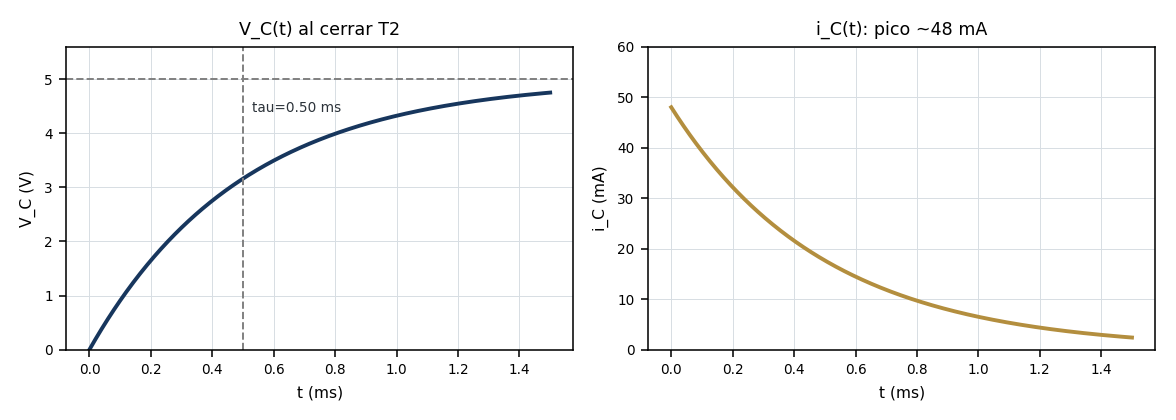
\includegraphics[width=0.70\textwidth]{figs/hard_sat_curvas.png}
  \end{center}
  \begin{itemize}
    \item \textbf{Arriba:} $V_C$ sube de 0 a 5 V en $\approx 3\tau = \SI{1.5}{\milli\second}$.
    \item \textbf{Abajo:} $i_C$ tiene un \textbf{pico de $\approx \SI{48}{\milli\ampere}$}
      al cerrar T2 y decae exponencialmente.
  \end{itemize}
\end{frame}

% ---------------------------------------------------------------------
\begin{frame}{6 · ¿Por qué saturación dura?}
  \begin{itemize}
    \item \textbf{Independencia de $\beta$:} con $\beta_{diseño}=10$ el transistor
      satura aunque el real tenga $\beta=50$–$300$ ($I_B$ de otra configuración no giraría).
    \item \textbf{Menos pérdidas:} $V_{CE,sat}\approx 0.2\,\mathrm{V}$
      $\Rightarrow P_{ON}=V_{CE,sat}\cdot I_C \approx 0.2\cdot 50\,\mathrm{mA}
      = \SI{10}{\milli\watt}$.
    \item \textbf{Rápido y predecible:} la corriente está limitada por $R_C$ y la carga $RC$.
    \item \textbf{Contra:} la base consume corriente; en señales muy pequeñas conviene un MOSFET.
  \end{itemize}
\end{frame}

% ---------------------------------------------------------------------
\begin{frame}{7 · Diseño alternativo: MOSFET en lugar de T2}
  \begin{itemize}
    \item Con un \textbf{NMOS} de nivel lógico ($V_{th}\le 2.1\,\mathrm{V}$) se hace
      la misma función \textbf{sin} consumir $I_B$: $I_G \approx 0$.
    \item La corriente de pico la sigue limitando el $100\,\mathrm{\Omega}$; el
      tiempo lo sigue mandando $\tau = R C$.
    \item Conmutador de \textbf{lado bajo} (fuente a GND) — igual que T2.
    \item Cambio de dimensionamiento: $V_{GS}$ vs $I_B$; ya no se usa la regla 10:1.
  \end{itemize}
\end{frame}

% ---------------------------------------------------------------------
\begin{frame}{Aplicación aeroespacial}
  \begin{itemize}
    \item Este tipo de conmutador se usa para \textbf{cargas capacitivas}:
      mantas térmicas, líneas de retenida de actuadores, buses auxiliares.
    \item El \textbf{pico de corriente} al encender debe dimensionarse (y a veces
      limitarse con el resistor en serie) para no dañar el bus ni el driver.
    \item Regla 10:1 da robustez frente a la variación de $\beta$ por temperatura
      ($\beta$ cambia en rango -40 °C a +85 °C — por eso "hard saturation" es la norma de diseño).
    \item En el vacío: verificar $P = V_{CE,sat} I_C$ y derating de cada etapa.
  \end{itemize}
\end{frame}

% ---------------------------------------------------------------------
\begin{frame}{Resumen del diseño}
  \begin{itemize}
    \item \textbf{T1} satura para entregar la base de \textbf{T2}; T2 en
      \textbf{saturación dura} por la regla \textbf{10:1}.
    \item Datos clave: $I_{C,max}=\SI{50}{\milli\ampere}$; $I_{B2,sat}=\SI{5}{\milli\ampere}$.
    \item La carga $RC$ ($100\,\mathrm{\Omega}$, $5\,\mathrm{\mu F}$) define
      $\tau=\SI{0.5}{\milli\second}$ y limita el pico a $\approx\SI{48}{\milli\ampere}$.
    \item El diseño es \textbf{predecible e independiente de $\beta$}; el MOSFET
      (semana 4) puede sustituir a T2 sin consumir base.
  \end{itemize}
\end{frame}

% ---------------------------------------------------------------------
\begin{frame}{Preguntas de verificación}
  \begin{enumerate}
    \item ¿Por qué diseñar con $\beta = 10$ (regla 10:1)?
      \uncover<2->{\emph{(Satura siempre, aunque $\beta$ real sea menor o varíe con la temperatura.)}}
    \item ¿Cuánto vale $I_{B2,sat}$ con $V_{CC}=5\,\mathrm{V}$ y $R_C=100\,\mathrm{\Omega}$?
      \uncover<3->{\emph{($I_{C,max}=50\,\mathrm{mA}\Rightarrow I_{B2,sat}=5\,\mathrm{mA}$.)}}
    \item ¿Cuál es el pico de corriente en el $100\,\mathrm{\Omega}$ de la carga?
      \uncover<4->{\emph{($\approx (5-0.2)/102.5 \approx \SI{47}{\milli\ampere}$.)}}
    \item ¿Qué define $\tau$ y qué velocidad tiene la carga?
      \uncover<5->{\emph{($\tau=RC=0.5\,\mathrm{ms}$; $t_{90\%}\approx 1.15\,\mathrm{ms}$.)}}
    \item ¿Qué ventaja tendría reemplazar T2 por un NMOS?
      \uncover<6->{\emph{(No consume corriente de base ($I_G\approx0$); se controla con tensión.)}}
  \end{enumerate}
\end{frame}

\end{document}
